\section{Rešenje problema}
\subsection{Opis rešenja problema}

Na osnovu analize \textit{D64 fajla} ustanovljeno je da se višestrukim čitanjem iste \textit{5.25 flopi diskete} dobijaju fajlovi sa greškama na različitim sektorima. Na osnovu ovoga konstruisano je rešenje gore opisanog problema koje je zasnovano na kombinaciji više \textit{D64 fajlova} sa ciljem da se kreira novi fajl koji bi imao manje ili u idealnom slučaju bio  bez grešaka. Suština postupka bi bila da se sektori koji imaju grešku zamene sa ispravnim sektoirma iz drugih \textit{D64 fajlova} iste \textit{5.25 flopi diskete} ukoliko oni postoje.

\subsection{Programsko rešenja problema}

Pošto svi fajlovi koji učestvuju u procesu imaju greške, algoritam počinje traženjem fajla koji ima najmanje grešaka jer to dalje smanjuje broj pretraga prilikom zamene sektora sa greškama. Dat je kod koji se bavi ovim procesom, gde se prvo učitavaju svi bajtovi tekućeg fajla i zatim u zavisnosti od dimenzija vrši se prebrojavanje sektora pod greškama i ukoliko taj fajl ima manje grešaka od trenutno najboljeg on se postavlja za novi najbolji. Postupak se ponavlja  po principu traženja minimuma odnosno fajla sa najmanje grešaka.

\begin{lstlisting}[language=Java]
byte[] newFile = null;
int best = 1000;
for (File file : Singleton.getInstance().getCompare()
                                    .getCompare()) {
    byte[] fileContent = null;
    try {
    	fileContent = Files.readAllBytes(file
    	                           .toPath());
    } catch (IOException e1) {
    	// TODO Auto-generated catch block
    	e1.printStackTrace();
    }
    
    if(fileContent.length == 175531) {
    	int temp = 0;
    	for(int i=fileContent.length-1 ; 
    	 i > fileContent.length-684 ; i--) {
            if(fileContent[i] != 1) {
            	temp++;
            }
        }
    	if(temp <= best) {
    		best = temp;
    		newFile = fileContent;
    	}
    }else if(fileContent.length == 197376){
    	int temp = 0;
    	for(int i=fileContent.length-1 ; 
    	i > fileContent.length-769 ; i--) {
            if(fileContent[i] == 1) {
            }else {
            	temp++;
            }
        }
    	if(temp <= best) {
    		best = temp;
    		newFile = fileContent;
    	}
    }else if(fileContent.length == 196608 
            || fileContent.length == 174848)
    	newFile = fileContent;
    	best = -1;
    }	
    Singleton.getInstance().getCompare()
                   .setFiles(fileContent);
}
\end{lstlisting}

Po pronalasku fajla sa najmanje grešaka, prolaskom kroz bajtove koji govore o greškama nad sektorima, uzimajući redom sektore sa greškama, proveravamo da li postoji fajl u kome je taj sektor ispravan. Ukoliko postoji vrši se kopiranje bajtova ispravnog sektora u bajtove neispravnog. Ovaj postupak se nastavlja do poslednjeg sektora sa greškama i u idealnom slučaju rezultuje fajlom bez grešaka.Dat je kod koji se bavi ovim postpukom za fajlove koji oslikavaju \textit{5.25 flopi disketu} sa 35 traka dok je za 40 traka postupak zansovan na istom principu samo sa različitim brojem dodatnih bajtova za greške.

\begin{lstlisting}[language=Java]
for(int i=newFile.length-683 
    ; i < newFile.length-1 ; i++) {
if(newFile[i] != 1) {
	for (byte[] b : Singleton
	.getInstance()
	.getCompare().getFiles()) {
		if(b[i] == 1) {
			for(int j = (i-174848)*256;
			j < (i-174848)*256+256 ; j++) {
				newFile[j] 
				    = b[j];
			}
			newFile[i] = 1;
			break;
		}
	}
}
}
\end{lstlisting}

\subsection{Prikaz implementiranog rešenja}

Početni izgled aplikacije prikazan je na slici \ref{img:aplikacija}. Klikom na dugme \textit{Select D64} vršimo izbor fajlova. Klikom na dugme \textit{Fix selected D64} pokreće se gore opisani algoritam za popravku selektovanih fajlova i interno kreiranje novog sa minimalnim brojem grešaka. Klikom na dugme \textit{Save D64} omogućava se čuvanje prethodno popravljenog i prikazanog fajla na lokaciji koju korisnik odabere. Klikom na dugme \textit{Refresh} vrši se deselekcija svih selektovanih fajlova kao i selekcija fajlova za prikaz.

Selekcija fajlova se vrši na osnovu čekera u levom donjem delu aplikacije a prikaz na osnovu radio dugmadi. Brojevi kod vizuelnog prikaza govore o kojoj traci \textit{5.25 flopi diskete} je reč dok donja traka služi za prikaz svih informacija bitnih za korisnika. Izgled ovog dela aplikacije prikazan je na slici \ref{img:aplikacija1}.

\begin{figure}[ht]
\begin{center}
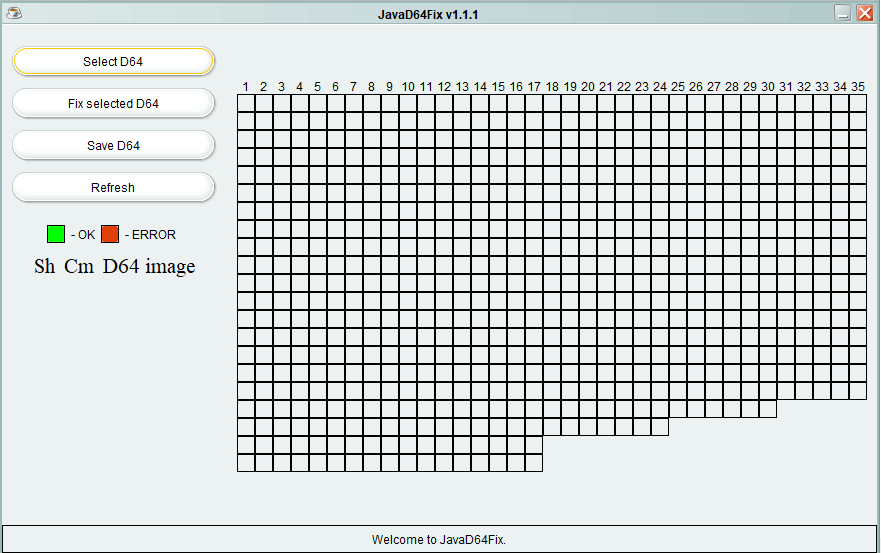
\includegraphics[width=\textwidth]{img/aplikacija.png}
\caption{Izgled aplikacije}
\label{img:aplikacija}
\end{center}
\end{figure}

\begin{figure}[ht]
\begin{center}
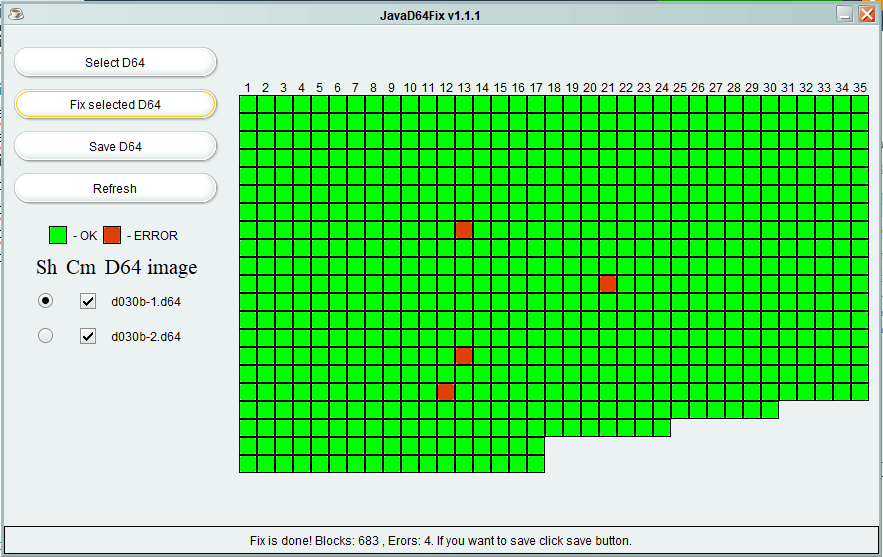
\includegraphics[width=\textwidth]{img/aplikacija1.png}
\caption{Izgled aplikacije}
\label{img:aplikacija1}
\end{center}
\end{figure}
